% Generator: hand-authored TikZ schematic traced from the fixed source; ellipse and chord coordinates are illustrative.
% Source ID: src-120ea104f8cb373f5731039fa9d36469df457869849f27420831962ef1ad2306
% PDF SHA-256: d0081500bd56d03199ddcf232fe8e870f2ecd7e9c41ba849417af9af79fbb702
% PDF page 2; printed page 125; question 18.
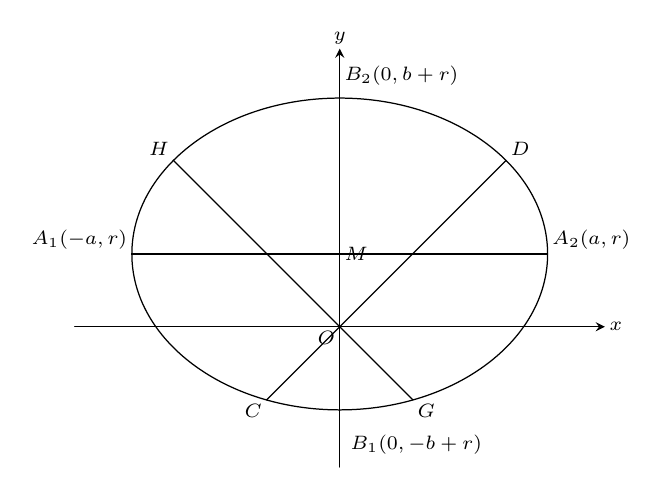
\begin{tikzpicture}[
  x=0.66cm,y=0.66cm,line width=0.45pt,line cap=round,>=stealth,
  every node/.style={font=\scriptsize,inner sep=1.5pt}
]
  \coordinate (O)  at (0,0);
  \coordinate (M)  at (0,1.4);
  \coordinate (A1) at (-4,1.4);
  \coordinate (A2) at (4,1.4);
  \coordinate (B1) at (0,-1.6);
  \coordinate (B2) at (0,4.4);
  \coordinate (H)  at (-3.2,3.2);
  \coordinate (G)  at (1.408,-1.408);
  \coordinate (C)  at (-1.408,-1.408);
  \coordinate (D)  at (3.2,3.2);

  \draw[->] (-5.1,0)--(5.1,0) node[right] {$x$};
  \draw[->] (0,-2.7)--(0,5.35) node[above] {$y$};
  \draw (M) ellipse [x radius=4,y radius=3];
  \draw (A1)--(A2);
  \draw (H)--(G) (C)--(D);

  \node[above left] at (A1) {$A_1(-a,r)$};
  \node[above right] at (A2) {$A_2(a,r)$};
  \node[above right] at (0,4.55) {$B_2(0,b+r)$};
  \node[below right] at (0.12,-2.0) {$B_1(0,-b+r)$};
  \node[right] at (M) {$M$};
  \node[below left] at (O) {$O$};
  \node[above left] at (H) {$H$};
  \node[below right] at (G) {$G$};
  \node[below left] at (C) {$C$};
  \node[above right] at (D) {$D$};
\end{tikzpicture}
